\documentclass[11pt]{article}\usepackage[]{graphicx}\usepackage[]{color}
% maxwidth is the original width if it is less than linewidth
% otherwise use linewidth (to make sure the graphics do not exceed the margin)
\makeatletter
\def\maxwidth{ %
  \ifdim\Gin@nat@width>\linewidth
    \linewidth
  \else
    \Gin@nat@width
  \fi
}
\makeatother

\definecolor{fgcolor}{rgb}{0.345, 0.345, 0.345}
\newcommand{\hlnum}[1]{\textcolor[rgb]{0.686,0.059,0.569}{#1}}%
\newcommand{\hlstr}[1]{\textcolor[rgb]{0.192,0.494,0.8}{#1}}%
\newcommand{\hlcom}[1]{\textcolor[rgb]{0.678,0.584,0.686}{\textit{#1}}}%
\newcommand{\hlopt}[1]{\textcolor[rgb]{0,0,0}{#1}}%
\newcommand{\hlstd}[1]{\textcolor[rgb]{0.345,0.345,0.345}{#1}}%
\newcommand{\hlkwa}[1]{\textcolor[rgb]{0.161,0.373,0.58}{\textbf{#1}}}%
\newcommand{\hlkwb}[1]{\textcolor[rgb]{0.69,0.353,0.396}{#1}}%
\newcommand{\hlkwc}[1]{\textcolor[rgb]{0.333,0.667,0.333}{#1}}%
\newcommand{\hlkwd}[1]{\textcolor[rgb]{0.737,0.353,0.396}{\textbf{#1}}}%
\let\hlipl\hlkwb

\usepackage{framed}
\makeatletter
\newenvironment{kframe}{%
 \def\at@end@of@kframe{}%
 \ifinner\ifhmode%
  \def\at@end@of@kframe{\end{minipage}}%
  \begin{minipage}{\columnwidth}%
 \fi\fi%
 \def\FrameCommand##1{\hskip\@totalleftmargin \hskip-\fboxsep
 \colorbox{shadecolor}{##1}\hskip-\fboxsep
     % There is no \\@totalrightmargin, so:
     \hskip-\linewidth \hskip-\@totalleftmargin \hskip\columnwidth}%
 \MakeFramed {\advance\hsize-\width
   \@totalleftmargin\z@ \linewidth\hsize
   \@setminipage}}%
 {\par\unskip\endMakeFramed%
 \at@end@of@kframe}
\makeatother

\definecolor{shadecolor}{rgb}{.97, .97, .97}
\definecolor{messagecolor}{rgb}{0, 0, 0}
\definecolor{warningcolor}{rgb}{1, 0, 1}
\definecolor{errorcolor}{rgb}{1, 0, 0}
\newenvironment{knitrout}{}{} % an empty environment to be redefined in TeX

\usepackage{alltt}

\usepackage{amsmath,graphicx}
\usepackage[margin=.9in]{geometry}
\usepackage{parskip} % no indentation
\usepackage{array}
% \usepackage{enumitem}
\usepackage{enumerate}
\usepackage{changepage} % for adjustwidth
\usepackage{array}
\usepackage{booktabs}
\usepackage{multicol}
\IfFileExists{upquote.sty}{\usepackage{upquote}}{}
\begin{document}

{\Large \bf Introduction to Markov Chains}\\[1ex]
{\large \bf Stat 340, Fall 2021}


{\bf Example.\footnote{Source: Introduction to Stochastic Processes with R by Bob Dobrow}}
University administrators have developed a Markov chain model to simulate graduation rates at their school. Students might drop out, repeat a year, or move on to the next year. Below is a graph representing the possible transitions that students can make at the university. Probabilities are listed next to each possible path, and only paths with positive probability are drawn.

\begin{knitrout}
\definecolor{shadecolor}{rgb}{0.969, 0.969, 0.969}\color{fgcolor}

{\centering 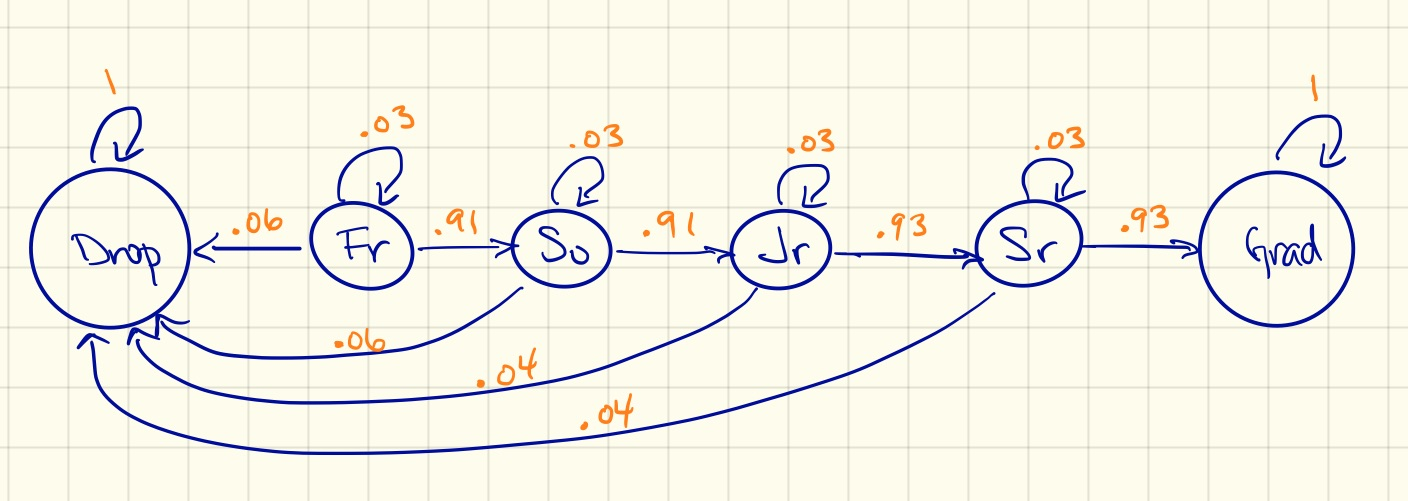
\includegraphics[width=0.9\linewidth]{figs/graduation_mc} 

}


\end{knitrout}



{\bf Your turn:}

\begin{enumerate}

\item What's the probability that a student who drops out will re-enroll?\\[0.25in]

\item What's the probability that a senior will graduate?\\[0.25in]

\item Does that probability depend on how many years it took them to achieve senior class standing?\\[0.25in]

\end{enumerate}


{\bf Definition: Markov chain}

A sequence of random variables, $X_0, X_1, X_2, \ldots$, taking values in the \emph{state space} $\lbrace 1, \ldots, M \rbrace$ is called a Markov chain if for all $n \ge 0$\\[0.9in]

Remarks:

\begin{itemize}
 
\item Think of $X_n$ as the state of the system at (discrete) time $n$. 

\item $q_{ij}$ is the \emph{transition probability} from state $i$ to state $j$.

\end{itemize}

\clearpage

{\bf Definition: Transition matrix}

A Markov chain can be represented by an $M \times M$ matrix of the probabilities $Q = \left( q_{ij} \right)$

\bigskip

where the rows represent the

\bigskip
and the columns represent the


\bigskip

{\bf Your turn:} Write down the $6 \times 6$ transition matrix for the university graduation rate Markov chain model.\\[3in]


\begin{enumerate}
\setcounter{enumi}{3}
\item Should the probabilities within each row sum to 1?\\[0.5in]
\item Should the probabilities within each row sum to 1?\\[0.6in]
\end{enumerate}

{\bf Calculating probabilities using the transition matrix}

If we know the transition matrix, $Q$, then we can derive the probability that a student goes from state $i$ to state $j$ in some given number of steps.

\bigskip
\bigskip

One-step transition probability: $P(X_{n+1} = j | X_n = i ) =$

\clearpage

Two-step transition probability: $P(X_{n+2} = j | X_n = i ) =$\\[2.5in]

$m$-step transition probability: $P(X_{n+m} = j | X_n = i ) =$

\bigskip
\bigskip

{\bf Marginal distribution of $\bf X_n$}

Suppose that at time $n$, $X_n$ has PMF given by ${\bf s} = (s_1, s_2, \ldots, s_m)$ where $s_i = P(X_n = i)$.\\

We can use the law of total probability to derive the PMF of $X_{n+1}$:\\[2.5in]

{\bf Uses of Markov Chains}\\

\begin{enumerate}
\item Use a Markov chain model, if your Markov chain is a reasonable abstraction of reality.\\

\item {\bf Markov Chain Monte Carlo (MCMC)}. Synthetically construct a Markov chain that is {\emph known} to converge to the distribution of interest.\\
\end{enumerate}

Not all Markov chains will converge to a single distribution, so we need a few more concepts before we can explore MCMC.

\clearpage

{\bf Classification of states}

{\bf Definition:} A state is {\bf recurrent} if starting there, the chain has probability 1 of returning to that state.\\

{\bf Definition:} A state that is not recurrent is {\bf transient}.\\

{\bf Definition:} If it's possible to get from any state to any state in a chain (with positive probability) \emph{in a finite number of steps}, then  it is {\bf irreducible}.\\

{\bf Definition:} A chain that is not irreducible is {\bf reducible}.\\


{\bf Your turn:} Assume that each of the Markov chains given below have uniform transition probabilities. For each Markov chain

\begin{enumerate}[i.]
\item Classify the chain as reducible or irreducible
\item Identify the transient states
\item Identify the recurrent states
\end{enumerate}

\begin{multicols}{2}

\begin{knitrout}
\definecolor{shadecolor}{rgb}{0.969, 0.969, 0.969}\color{fgcolor}
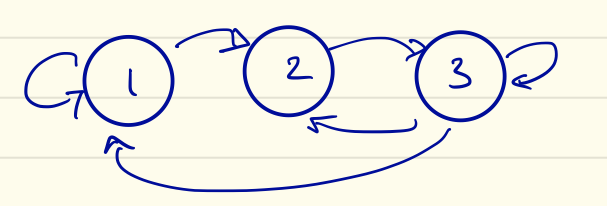
\includegraphics[width=\maxwidth]{figs/mc1} 
\end{knitrout}

\vspace{1.15in}

\begin{knitrout}
\definecolor{shadecolor}{rgb}{0.969, 0.969, 0.969}\color{fgcolor}
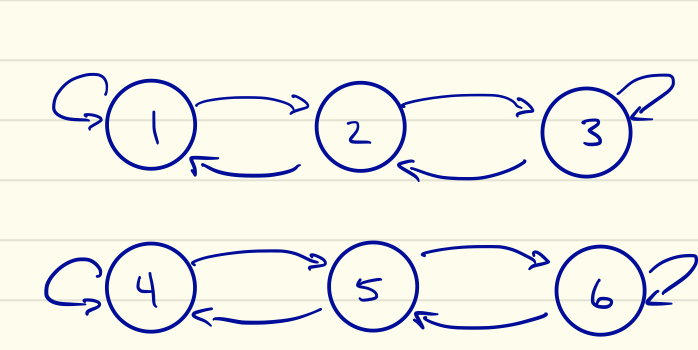
\includegraphics[width=\maxwidth]{figs/mc2} 
\end{knitrout}

\vspace{1.15in}

\begin{knitrout}
\definecolor{shadecolor}{rgb}{0.969, 0.969, 0.969}\color{fgcolor}
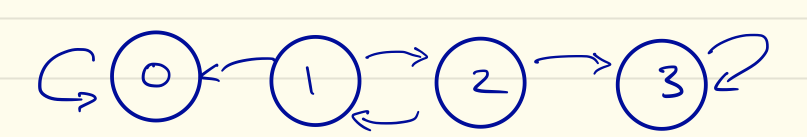
\includegraphics[width=\maxwidth]{figs/mc3} 
\end{knitrout}

\vspace{1.75in}

\begin{knitrout}
\definecolor{shadecolor}{rgb}{0.969, 0.969, 0.969}\color{fgcolor}

{\centering 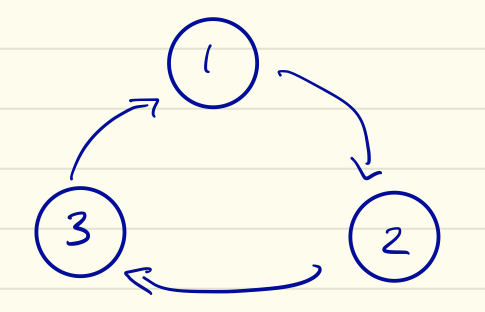
\includegraphics[width=0.6\linewidth]{figs/mc4} 

}


\end{knitrout}

\vspace{1.15in}

\end{multicols}

\clearpage


{\bf Long-run behavior}

{\bf Definition.} For irreducible, aperiodic Markov chains, the fraction of the time spent in each of the recurrent states is given by the {\bf stationary distribution.} (a.k.a. steady state)

\bigskip

${\bf s} = (s_1, s_2, \ldots, s_m)$ is a stationary distribution if

\bigskip
\bigskip

{\bf Key result:}  A Markov chain which starts out with a stationary distribution will stay in the stationary distribution forever.

\bigskip
\bigskip

{\bf Theorem.} For any irreducible Markov chain:

\begin{enumerate}
\item A stationary distribution exists.

\item The stationary distribution is unique.

\item $s_i = 1/ r_i$, where $r_i$ is the expected number of steps required to return to state $i$, if starting at state $i$.

\item If $Q^m$ is strictly positive (which implies aperiodic and recurrent) for some $m$, then

$$P(X_n = i) \to s_i \text{ as } n \to \infty$$


\end{enumerate}

\end{document}
